As intoduced in Chapter \ref{density_fitting_theory}
density fitting is ma method that attemps to reproduce the physical properties of a electron density produced by a set of orbitals by using a orbital free basis set.
In the following the different denisty fitting methods are introduced and compared.
\subsection{Metrics}
To evaluate the different density fitting methods the following metrics are used:
\begin{enumerate}
    \item Mean Absolute Error (MAE) of the Energies (Hartree, External, xc, kinetic)
    \item Mean Absolute Error (MAE) of the of the number of electrons $N = \int \rho(\mathbf{r}) d\mathbf{r}$
    \item The L2 Norm of the difference in densities $\text{L2}[\rho-\rho'] = \sqrt{\int (\rho(\mathbf{r})-\rho'(\mathbf{r}))^2} d\mathbf{r}$
    \item The L1 Norm of the difference in densities $\text{L1}[\rho-\rho'] = \int |\rho(\mathbf{r})-\rho'(\mathbf{r})| d\mathbf{r}$
    \item The Gradient of the total energy at the ground state (Interesting for convergence)
    \item The L1 Norm of negative values in the fitted density $\text{L1}[\rho'] = \int \text{RELU}(-\rho'(\mathbf{r})) d\mathbf{r}$
    \item The Hartree energy of the residual density $\text{Hartree}[\rho-\rho'] = \int \int \frac{(\rho(\mathbf{r})-\rho'(\mathbf{r}))(\rho(\mathbf{r'})-\rho'(\mathbf{r'}))}{|\mathbf{r}-\mathbf{r'}|}d\mathbf{r}d\mathbf{r'}$
    \item Stability of the fitted density coefficients (std of the coefficients)
\end{enumerate}
\subsection{Density fitting methods}
Here the different density fitting methods which were considert are introduced and compared.
The derivation are include in Appendix \ref{appendix:density_fitting}
\subsubsection{Overlap Density fitting}
\begin{align}
        \mathcal{L}(\mathbf{p}) &= \mathbf{p} W \mathbf{p} - 2 \mathbf{p}\bar { L} \bar\Gamma + \bar\Gamma \mathbf{D}\bar\Gamma
\end{align}

\subsubsection{Hartree Density fitting}
Minimizes the following metric:
\begin{align}
        \mathcal{L}(\mathbf{p}) &= \mathbf{p} \tilde{W} \mathbf{p} - 2 \mathbf{p}\bar {\tilde L} \bar\Gamma + \bar\Gamma \tilde{\mathbf{D}}\bar\Gamma
\end{align}
Which results in the following formula for the fitted density coefficients:
\begin{align}
    \mathbf{p}&=\tilde{W}^{-1}\bar {\tilde L} \bar\Gamma\\
\end{align}


\subsubsection{Hartree+External Density Fitting}
\begin{align}
        \mathcal{L}(\mathbf{p}) &= \mathbf{p} \tilde{W} \mathbf{p} - 2 \mathbf{p}\bar {\tilde L} \bar\Gamma + \bar\Gamma \tilde{\mathbf{D}}\bar\Gamma + (\mathbf{p}\mathbf{v}_{ext}-\bar\Gamma \bar{V}_{ext})^2
\end{align}
\begin{align}
    A&:=\tilde{W}+\mathbf{v}_{ext}\mathbf{v}_{ext}^T\\
    \mathbf{p}&:=A^{-1}\left(\bar {\tilde L}+\mathbf{v}_{ext}\bar{V}_{ext}\right) \bar\Gamma\\
\end{align}

\subsubsection{Hartree+External Density Fitting MOFDFT-Version}
\begin{align}
\mathcal{L}(\mathbf{p}) &= \mathbf{p} \tilde{W} \mathbf{p} - 2 \mathbf{p}\bar {\tilde L} \bar\Gamma + \bar\Gamma \tilde{\mathbf{D}}\bar\Gamma + (\mathbf{p}\mathbf{v}_{ext}-\bar\Gamma \bar{V}_{ext})^2\\
&\left(\begin{array}{c}\tilde{W}\\v_{ext}^T\end{array}\right) \mathbf{p} =  \left(\begin{array}{c}\tilde{L} \bar{\Gamma} \\ \bar{\Gamma}\bar{V}_{ext}\end{array}\right)
\end{align}


\subsubsection{Hartree+External Density Fitting with enforced electron number}
\begin{align}
    \mathcal{L}(\mathbf{p},\mu) &= \mathbf{p} \tilde{W} \mathbf{p} - 2 \mathbf{p}\bar {\tilde L} \bar\Gamma + (\mathbf{p}\mathbf{v}_{ext}-\bar\Gamma \bar{V}_{ext})^2+\mu(\mathbf{p}\mathbf{w}-\bar\Gamma\bar S)\\
    A^{-1}\left(\bar {\tilde L} + \mathbf{v}_{ext} \bar{V}_{ext}- \mathbf{w}\frac{\mathbf{w}A^{-1}\bar {\tilde L} +\mathbf{w}A^{-1}\mathbf{v}_{ext} \bar{V}_{ext}-\bar S}{\mathbf{w}A^{-1}\mathbf{w}}\right)\bar\Gamma\\
\end{align}



\subsubsection{Hartree Density Fitting with enforced electron number and enforced external energy}
\begin{align}
    \mathcal{L}(\mathbf{p},\mu,\nu) &= \mathbf{p} \tilde{W} \mathbf{p} - 2 \mathbf{p}\bar {\tilde L} \bar\Gamma + \nu(\mathbf{p}\mathbf{v}_{ext}-\bar\Gamma \bar{V}_{ext})+\mu(\mathbf{p}\mathbf{w}-\bar\Gamma\bar S)\\
\end{align}


\subsubsection{Hartree+External Density Fitting MOFDFT-Version with soft enforced electron number}
\begin{align}
    \mathcal{L}(\mathbf{p}) &= \mathbf{p} \tilde{W} \mathbf{p} - 2 \mathbf{p}\bar {\tilde L} \bar\Gamma + \bar\Gamma \tilde{\mathbf{D}}\bar\Gamma + (\mathbf{p}\mathbf{v}_{ext}-\bar\Gamma \bar{V}_{ext})^2 + (\mathbf{p}\mathbf{w}-\bar\Gamma \bar{S})^2
\end{align}
\begin{align}
    \left(\begin{array}{c}\tilde{W}\\\mathbf{v}_{ext}^T\\\mathbf{w}^T\end{array}\right) \mathbf{p} =  \left(\begin{array}{c}\tilde{L} \bar{\Gamma} \\ \bar{\Gamma}\bar{V}_{ext}\\\bar S\bar \Gamma\end{array}\right)
\end{align}


\subsubsection{Hartree+External Density Fitting MOFDFT-Version with hard enforced electron number}
\begin{align}
    \mathcal{L}(\mathbf{p}) &= \left\lVert\left(\begin{array}{c}\tilde{W}\\v_{ext}^T\end{array}\right) \mathbf{p} - \left(\begin{array}{c}\tilde{L} \bar{\Gamma} \\ \bar{\Gamma}\bar{V}_{ext}\end{array}\right)\right\rVert^2 + \lambda (\mathbf{w}\mathbf{p}-N)
\end{align}



\subsubsection{Overlap Density fitting with enforced electron number}
\begin{align}
    \mathcal{L}(\mathbf{p},\mu) &= \mathbf{p} \tilde{W} \mathbf{p} - 2 \mathbf{p}\bar {\tilde L} \bar\Gamma + (\mathbf{p}\mathbf{v}_{ext}-\bar\Gamma \bar{V}_{ext})^2+\mu(\mathbf{p}\mathbf{w}-\bar\Gamma\bar S)\\
    A^{-1}\left(\bar {\tilde L} + \mathbf{v}_{ext} \bar{V}_{ext}- \mathbf{w}\frac{\mathbf{w}A^{-1}\bar {\tilde L} +\mathbf{w}A^{-1}\mathbf{v}_{ext} \bar{V}_{ext}-\bar S}{\mathbf{w}A^{-1}\mathbf{w}}\right)\bar\Gamma\\
\end{align}



\subsubsection{Overlap Density fitting with enforced electron number and enforced external energy}
\begin{align}
    \mathcal{L}(\mathbf{p},\mu,\nu) &= \mathbf{p} \tilde{W} \mathbf{p} - 2 \mathbf{p}\bar {\tilde L} \bar\Gamma + \nu(\mathbf{p}\mathbf{v}_{ext}-\bar\Gamma \bar{V}_{ext})+\mu(\mathbf{p}\mathbf{w}-\bar\Gamma\bar S)\\
\end{align}

The following plot shows the difference of the metrics evaluated on the first 1000 Molecules of QM9.

Insert plot here

A more detailed Table of the found falues for the different values can be found in the appendix\cite appendix.

\begin{figure}[h]
    \centering
    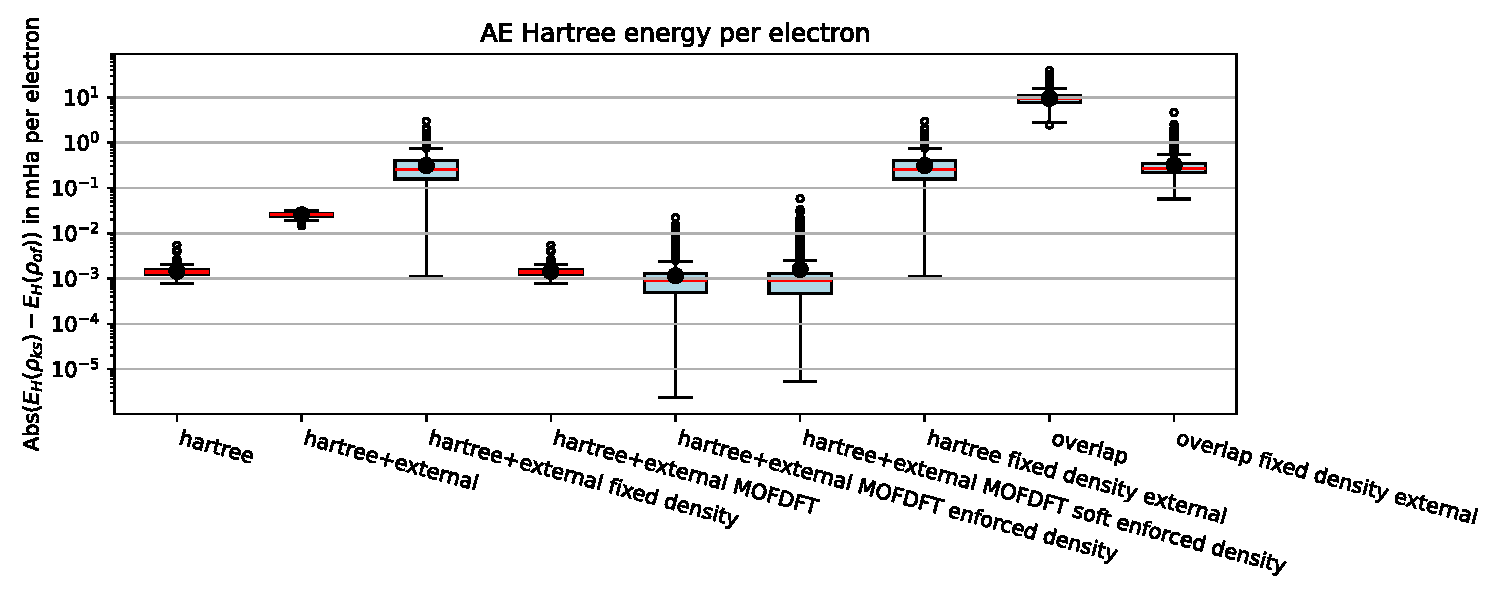
\includegraphics[width=0.5\textwidth]{chapters/results/results_images/AE_hartree_energy_on_even_tempered_2.5}
    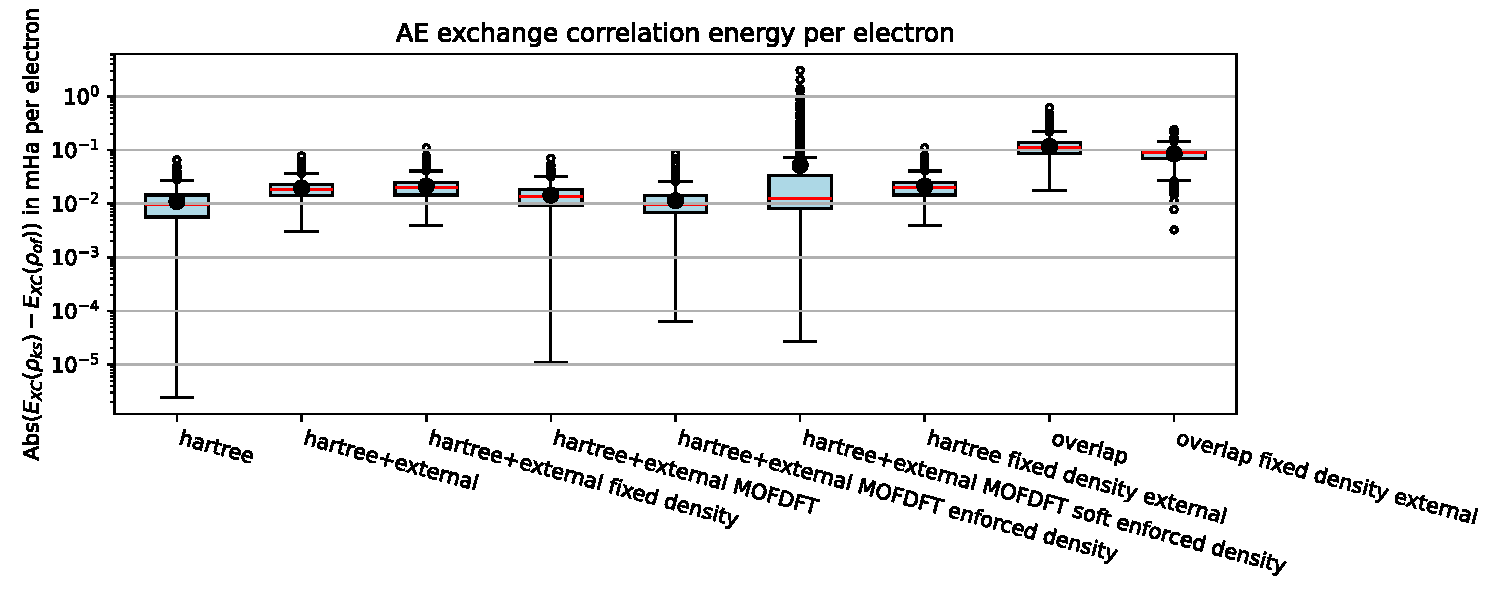
\includegraphics[width=.49\textwidth]{chapters/results/results_images/AE_xc_energy_on_even_tempered_2.5}
    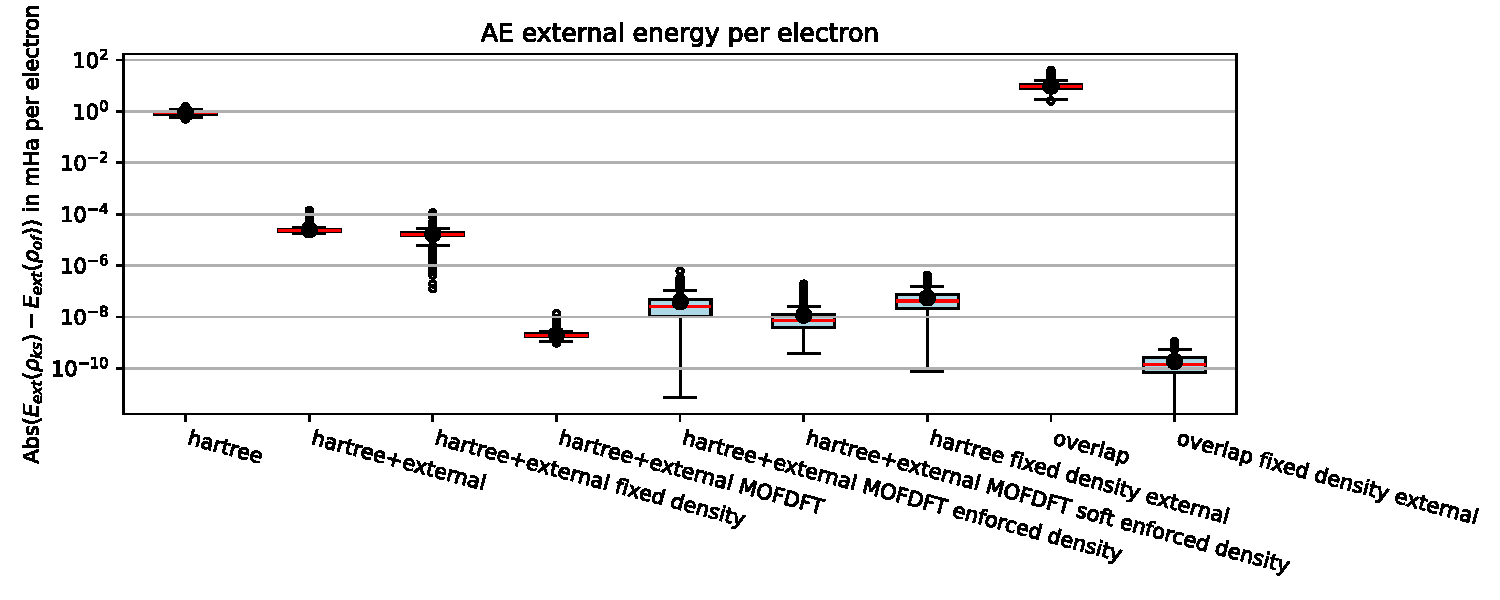
\includegraphics[width=.5\textwidth]{chapters/results/results_images/AE_ext_energy_on_even_tempered_2.5}
    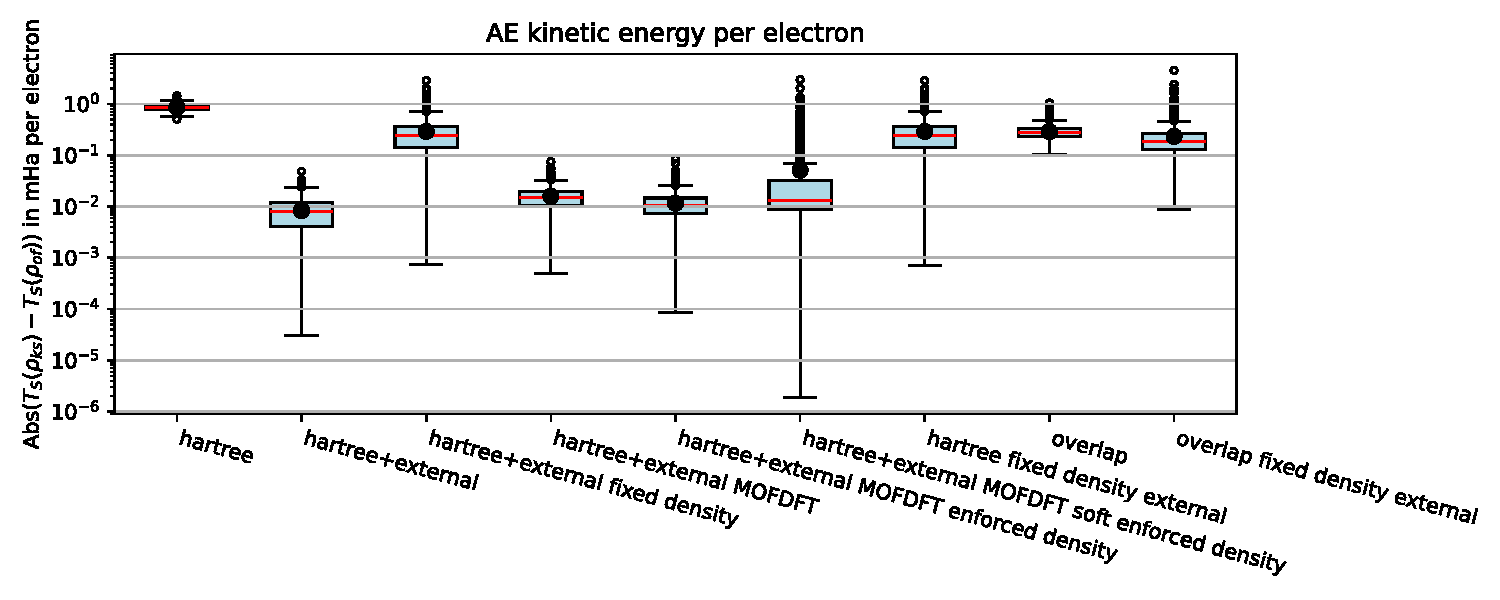
\includegraphics[width=.49\textwidth]{chapters/results/results_images/AE_kin_energy_on_even_tempered_2.5}
    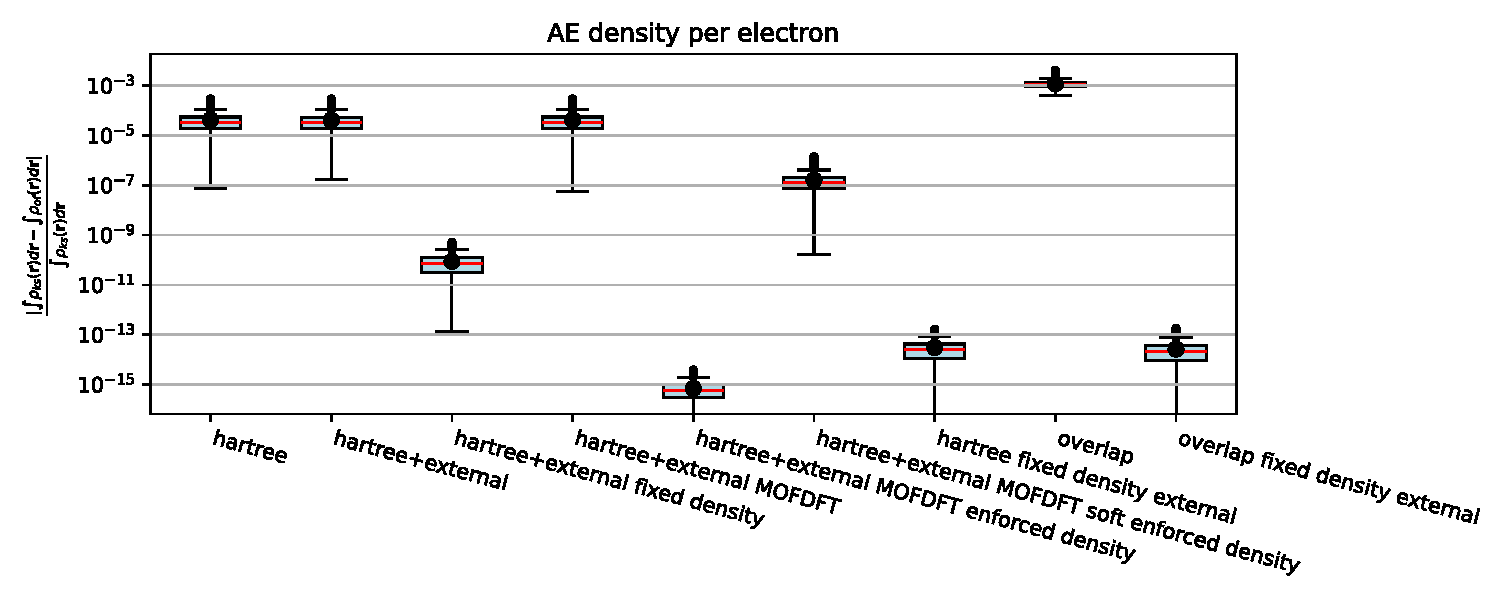
\includegraphics[width=.5\textwidth]{chapters/results/results_images/AE_density_on_even_tempered_2.5}
    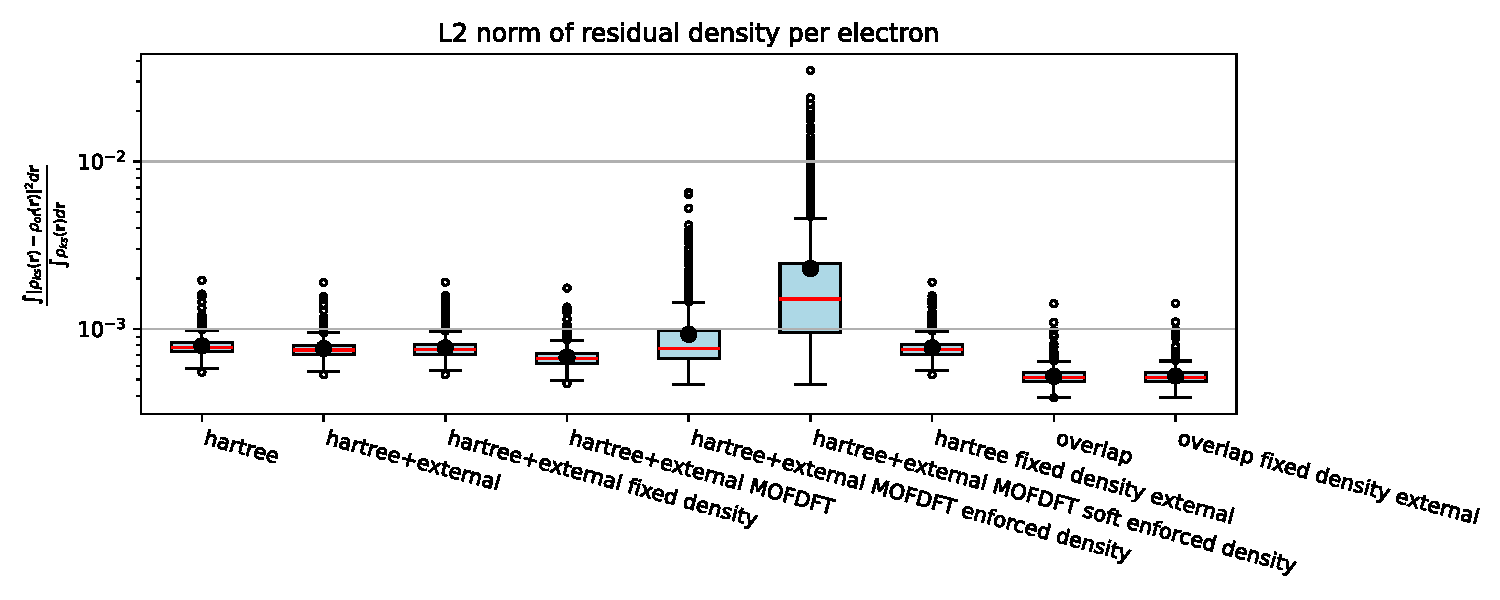
\includegraphics[width=0.49\textwidth]{chapters/results/results_images/L2_residual_densities_on_even_tempered_2.5}
    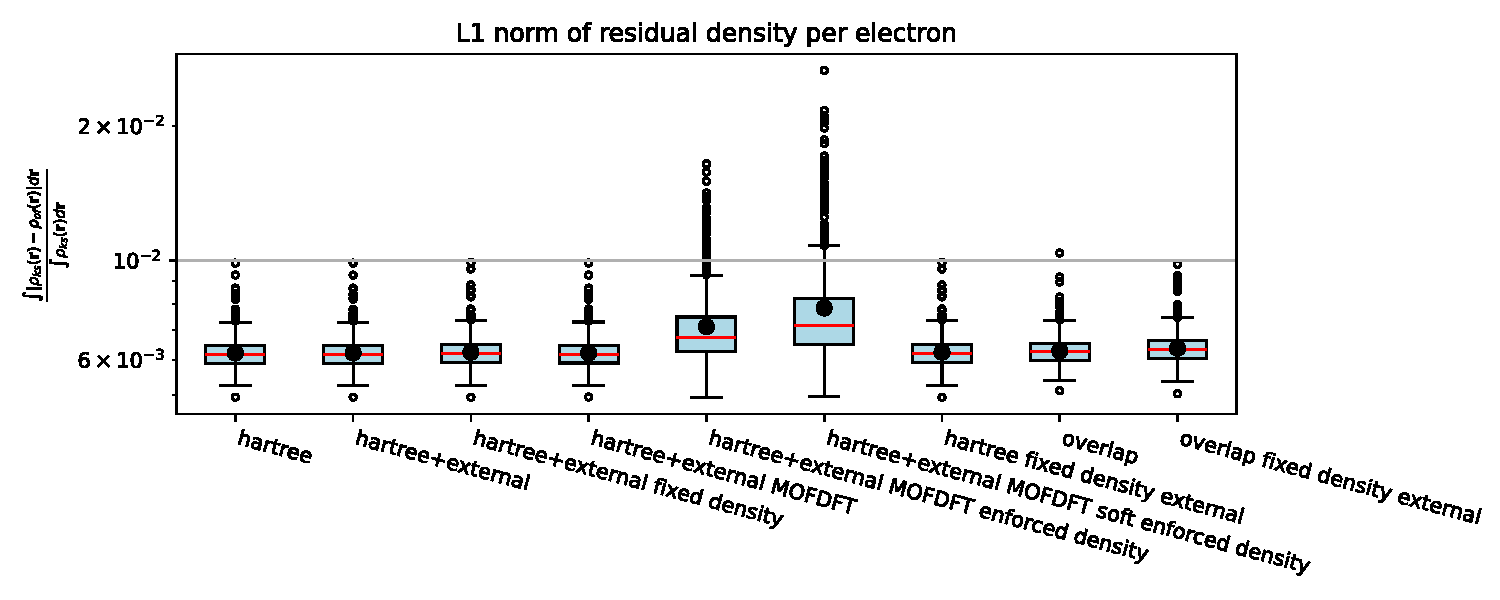
\includegraphics[width=0.5\textwidth]{chapters/results/results_images/L1_residual_densities_on_even_tempered_2.5}
    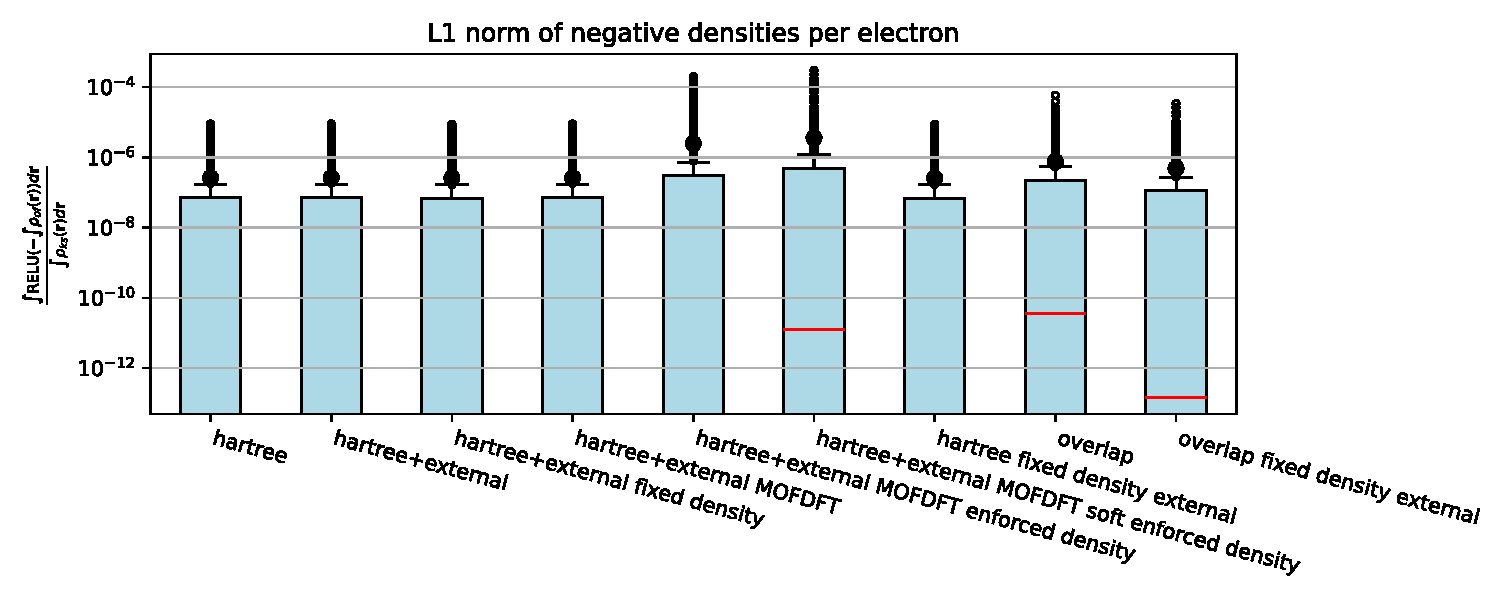
\includegraphics[width=0.49\textwidth]{chapters/results/results_images/L1_negative_densities_on_even_tempered_2.5}
    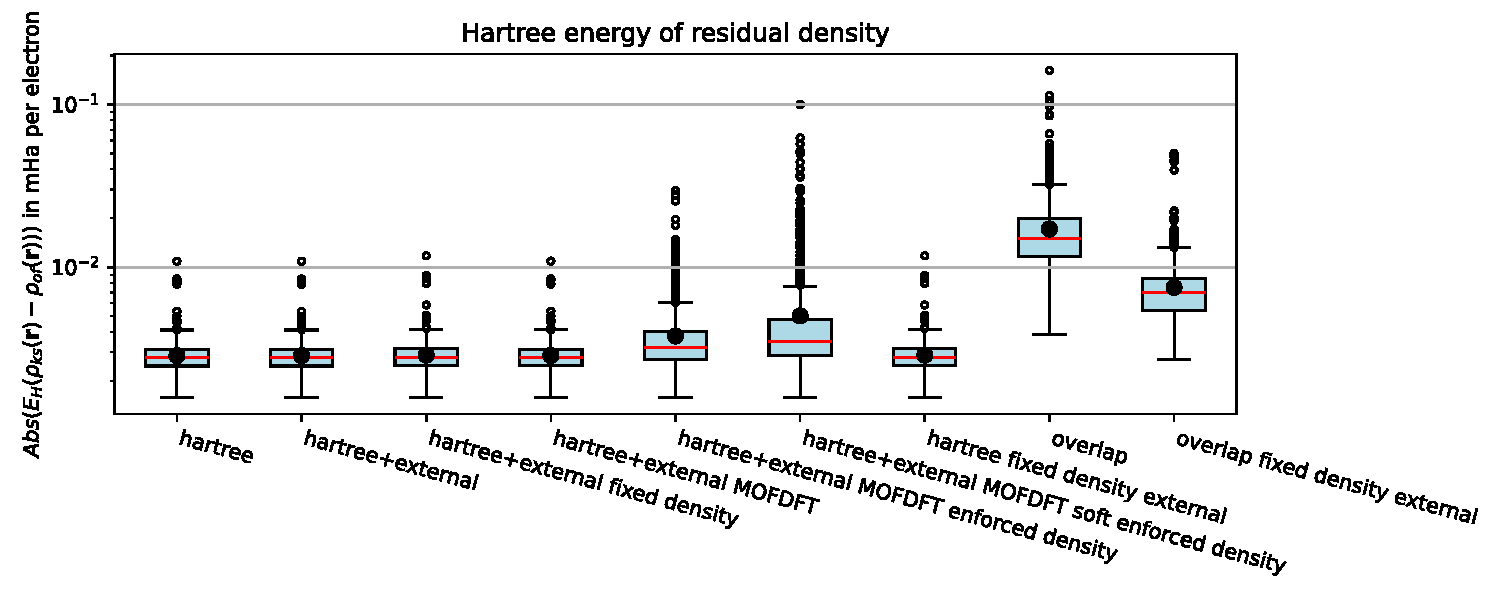
\includegraphics[width=0.5\textwidth]{chapters/results/results_images/L2_residual_hartree_on_even_tempered_2.5}
    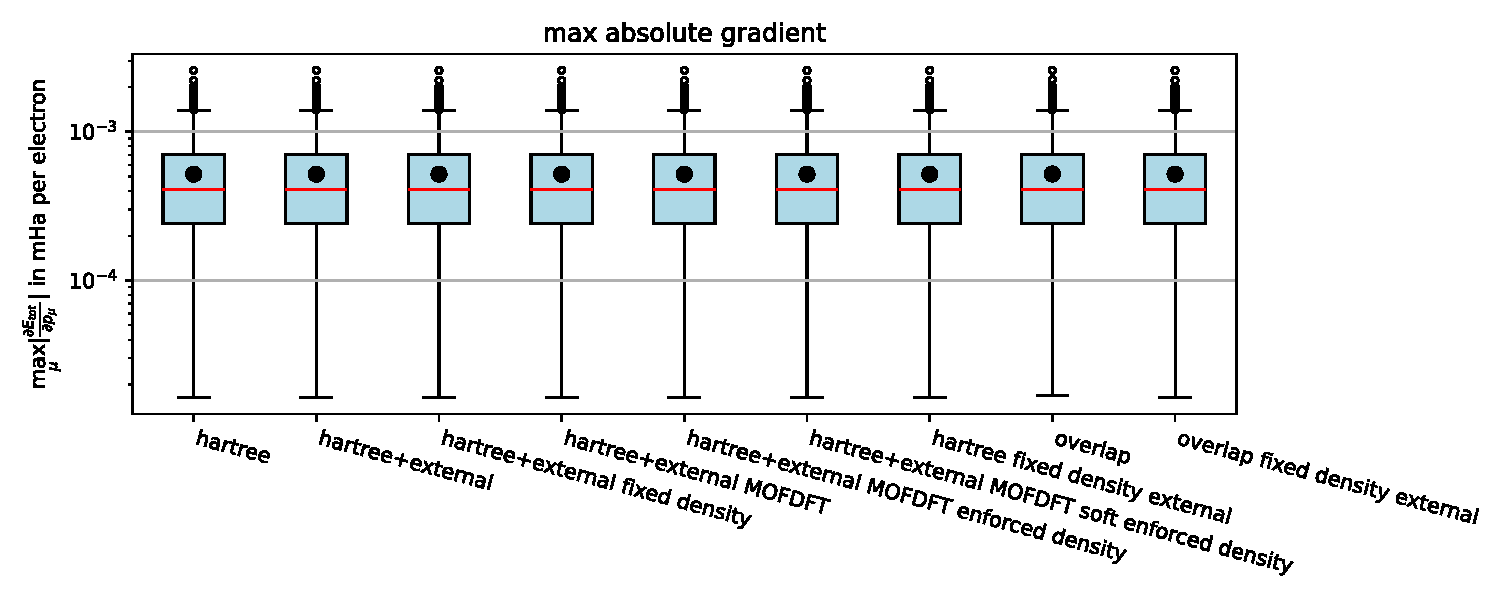
\includegraphics[width=0.49\textwidth]{chapters/results/results_images/max_abs_gradient_on_even_tempered_2.5}
    \includesvg[width=0.5\textwidth]{chapters/results/results_images/var_density_fitting}
    \caption{A plot of the different metrics evaluated on the first 1000 Molecules of the QM9 dataset}
    \label{fig:my_label}
\end{figure}

\begin{figure}[h]
    \centering
    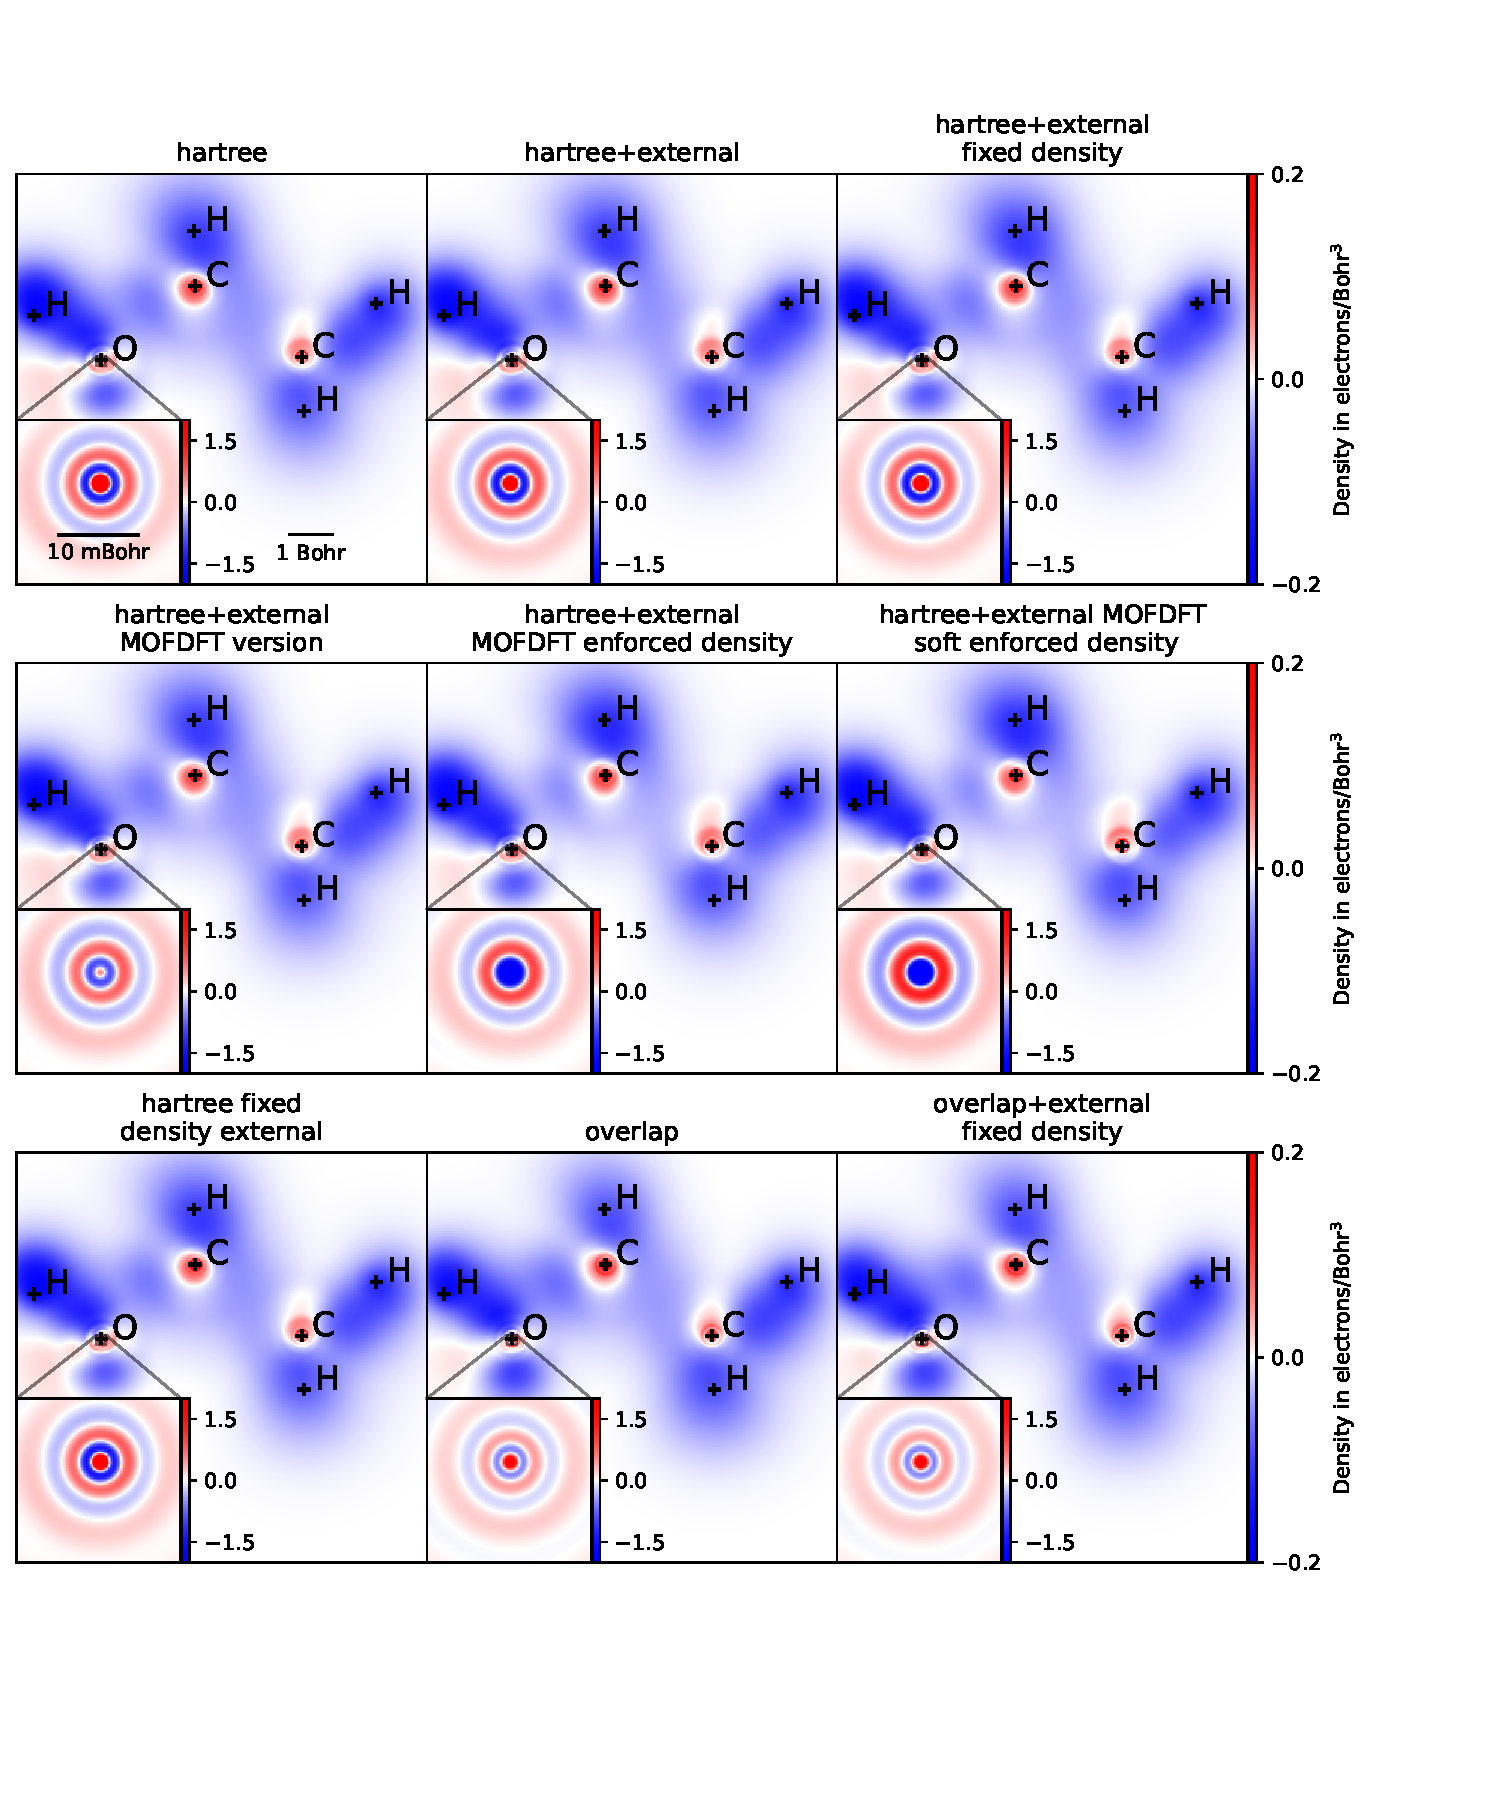
\includegraphics[width=1\textwidth]{chapters/results/results_images/density_fitting_slices}
    \caption{A plot of the different metrics evaluated on the first 1000 Molecules of the QM9 dataset}
    \label{fig:my_label2}
\end{figure}







